\documentclass[12pt,a4paper,onecolumn]{article}

%%%%%%%%%%%%%%%%%%%%%%%%%%%%%%%%%%%
% PAQUETES
%%%%%%%%%%%%%%%%%%%%%%%%%%%%%%%%%%%

\usepackage[margin=1in]{geometry}
\usepackage{authblk}
\usepackage[utf8]{inputenc}  % UTF-8 evita problemas de caracteres
\usepackage[T1]{fontenc}     % Mejor soporte de fuentes en LaTeX
\usepackage[spanish]{babel}  % Manejo correcto de idioma español
\usepackage{amsfonts}
\usepackage{graphicx} % Necesario para incluir imágenes
\usepackage{xcolor}
\usepackage{amsmath}
\usepackage{amssymb}
\usepackage[table]{xcolor}
\usepackage{setspace}
\usepackage{booktabs}
\usepackage{dcolumn}
\usepackage{rotating}
\usepackage{threeparttable}
\usepackage[capposition=top]{floatrow}
\usepackage[labelsep=period]{caption}
\usepackage{subcaption}
\usepackage{multicol}
\usepackage[bottom]{footmisc}
\usepackage{enumerate}
\usepackage{units}
\usepackage{placeins}
\usepackage{booktabs,multirow}
\usepackage{float}
\usepackage{pdflscape}      % Para landscape completo
\usepackage{lscape}         % Alternativa si pdflscape da problemas
\usepackage{longtable}      % Para tablas que ocupan más de una página
\usepackage{geometry}       % Para ajustar márgenes si es necesario

% Bibliografía
\usepackage{natbib}
\bibliographystyle{apalike}
\bibpunct{(}{)}{,}{a}{,}{,}

% Formato de párrafos
\renewcommand{\baselinestretch}{1}

% Definir columnas para tablas
\usepackage{array}
\newcolumntype{L}[1]{>{\raggedright\let\newline\\\arraybackslash\hspace{0pt}}m{#1}}
\newcolumntype{C}[1]{>{\centering\let\newline\\\arraybackslash\hspace{0pt}}m{#1}}
\newcolumntype{R}[1]{>{\raggedleft\let\newline\\\arraybackslash\hspace{0pt}}m{#1}}

\usepackage{xfrac}
\usepackage{bbold}

\setcounter{secnumdepth}{6}

\usepackage{titlesec}
\titleformat*{\subsection}{\normalsize \bfseries}

\usepackage[colorlinks=true,linkcolor=black,urlcolor=blue,citecolor=blue]{hyperref}

%%%%%%%%%%%%%%%%%%%%%%%%%%%%%%%%%%%
%     TÍTULO, AUTORES Y FECHA              %
%%%%%%%%%%%%%%%%%%%%%%%%%%%%%%%%%%%

\title{\textbf{Taller 2 - Predicción de Pobreza en Colombia}}

\author{%
\begin{center}
Harold Stiven Acuña\\
José David Cuervo\\
José David Dávila\\
César Augusto Alfaro
\end{center}%
}

\date{\today}

% Configuración simple para espaciado de párrafos
\setlength{\parskip}{0.6em} % Espacio entre párrafos
\setlength{\parindent}{1em} % Sangría moderada

\begin{document}

\maketitle
\thispagestyle{empty}

%%%%%%%%%%%%%%%%%%%%%%%%%%%%%%%%%%%
% ABSTRACT
%%%%%%%%%%%%%%%%%%%%%%%%%%%%%%%%%%%

\begin{abstract}
Este documento presenta el análisis de datos y la implementación de modelos de clasificación para la predicción de la pobreza en Colombia.
\end{abstract}

\medskip

\begin{flushleft}
    {\bf Palabras clave:} pobreza, clasificación, aprendizaje automático \\
    {\bf Clasificación JEL:} J31, C53, J16
\end{flushleft}

% Añadir información del repositorio GitHub
\begin{center}
    \textit{Repositorio GitHub:} \url{https://github.com/alfarocesar/BDML_Predicting_Poverty_Equipo8}
\end{center}

\pagebreak
\singlespacing
\setlength{\parindent}{0pt}
\setlength{\parskip}{1em}

%%%%%%%%%%%%%%%%%%%%%%%%%%%%%%%%%%%
%           DOCUMENTO                       %
%%%%%%%%%%%%%%%%%%%%%%%%%%%%%%%%%%%

\section{Introducción}

La migración del campo a la ciudad, producto de la Primera y Segunda Revolución Industrial, trajo consigo un aumento significativo de la población, así como conflictos de orden político, económico y social, en igual medida para todos los países que decidieron sumarse a dicho proceso de transformación emergente, como Gran Bretaña, Francia, Alemania, Estados Unidos, entre otros. Es así como la pobreza, como concepto abstracto y simbólico, se introduce en la discusión del mundo científico, mismo que se encontraba en auge, no solo para las ciencias exactas que derivan de las leyes de la física, sino también en ciencias cuyo objeto de estudio resultaba más abstracto y retador, aún en nuestros tiempos: la sociedad.

La pobreza, entonces, generó la inminente necesidad de ser considerada, sobre todo, para encontrar formas de medición acertadas. La razón de ser de ello es muy sencilla: a medida que la sociedad avanzaba, el discurso de los derechos se hizo más fuerte; la dignidad, el mínimo vital, el contrato social, entre otros, se hicieron vigentes y, en consecuencia, la pobreza se convirtió en objeto de estudio, con el propósito de determinar su existencia, evolución y distribución.

En este punto, la medición de la pobreza adquiere especial relevancia y su análisis, con el paso del tiempo, ha incluido inferencia, teoría, estadística, abstracción, idealización, predicción, cálculo y construcción de instrumentos \cite{tal2016measuring}. Sin embargo, aún falta teoría y una estructura definida que permita a los investigadores concluir que determinada asignación numérica representa adecuadamente la característica de la pobreza que se pretende medir \cite{huffman2024measurement}.

Amartya Sen señala que la pobreza se mide no solo frente a la falta de ingresos y recursos, sino también en la falta de capacidades que restringen las opciones y oportunidades de las personas. Así las cosas, sobrevienen dos dificultades hasta el momento: la falta de una estructura para medir la pobreza y la determinación de las características que representan dicha pobreza.

Una medición precisa, eficiente y oportuna de la pobreza es clave para diseñar políticas públicas que sean no solo efectivas, sino también costo-eficientes. Sin embargo, los métodos tradicionales de medición —basados en encuestas extensas— implican altos costos y tiempos prolongados de recolección, procesamiento y análisis. En respuesta a esta limitación, el uso de técnicas de \textit{machine learning} ofrece una alternativa prometedora: construir modelos que permitan predecir la condición de pobreza de los hogares utilizando un número reducido de variables y, en consecuencia, realizar evaluaciones más rápidas y baratas.

Este proyecto busca desarrollar modelos de clasificación binaria que permitan identificar si un hogar colombiano se encuentra en condición de pobreza, utilizando microdatos del DANE y la Misión MESE, a nivel de hogar e individuo. La Figura~\ref{fig:pobreza_colombia} ilustra la evolución reciente de la pobreza en el país, motivando así la necesidad de mejorar las herramientas de diagnóstico.

\begin{figure}[H]
  \centering
  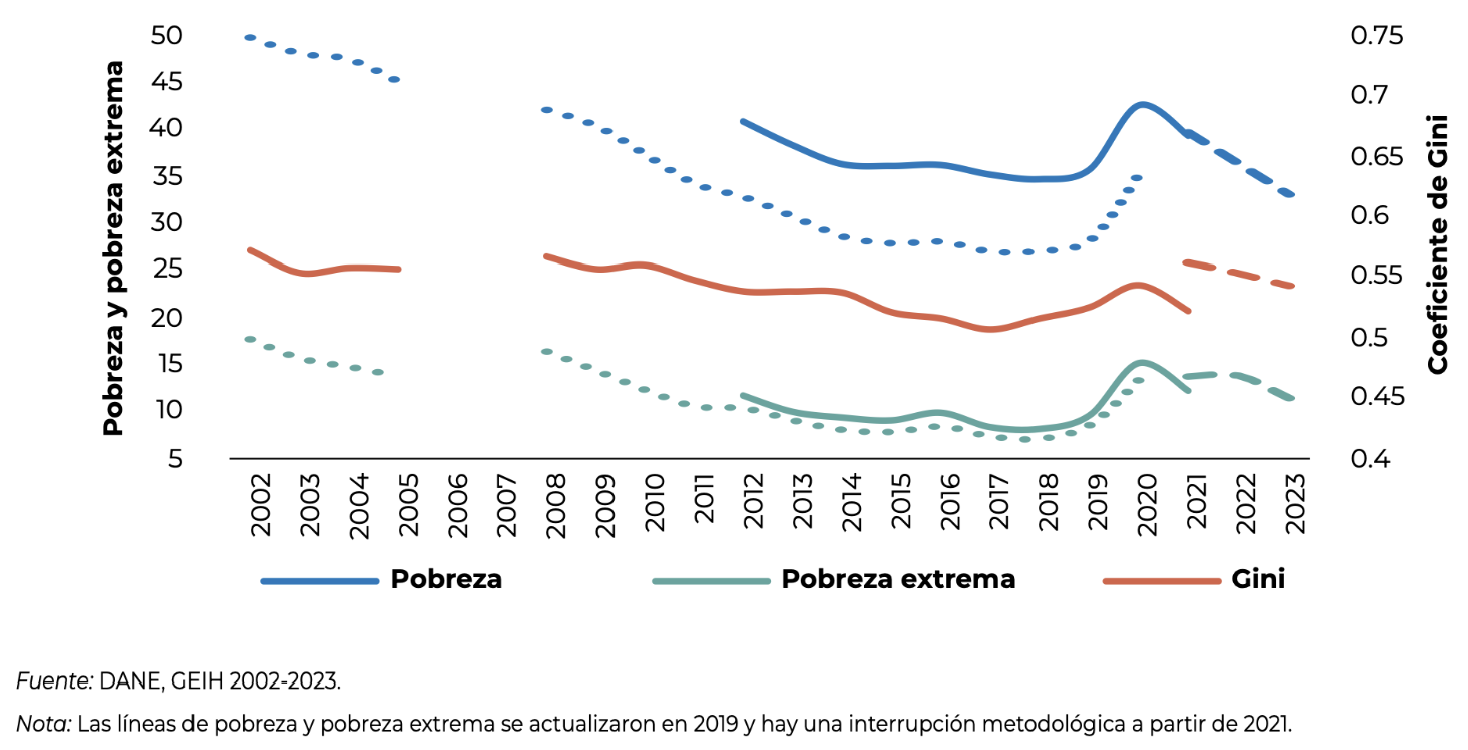
\includegraphics[width=0.85\textwidth]{../views/figures/pobreza_colombia.png}
  \caption{Evolución reciente de la pobreza monetaria en Colombia.}
  \label{fig:pobreza_colombia}
\end{figure}

A lo largo del documento se evalúan diferentes algoritmos de clasificación (como regresión logística, árboles de decisión, random forest, entre otros) y se presenta una comparación sistemática de su desempeño. El modelo con mejor rendimiento logró una puntuación F1 de \textbf{[0.5686]}, utilizando solo \textbf{[número]} variables, lo que representa un avance en términos de precisión y simplicidad. Este modelo fue seleccionado como la base para las predicciones entregadas en Kaggle.

Además de identificar el mejor algoritmo, se discute la importancia relativa de las variables predictoras, destacando aquellas con mayor capacidad explicativa. Estos hallazgos permiten no solo mejorar la focalización de políticas sociales, sino también abrir camino para sistemas de monitoreo más ágiles y adaptativos.

\section{Datos}
\subsection{Adecuación de los datos}

Los datos utilizados en este estudio provienen de DANE y la misión "Empalme de las Series de Empleo, Pobreza y Desigualdad (MESE)". Estos datos son adecuados para resolver el problema de predicción de pobreza por varias razones. Primero, contienen información detallada a nivel de hogar e individuo, lo que permite capturar la heterogeneidad socioeconómica de la población colombiana. Segundo, incluyen la variable objetivo de interés (Pobre) que está correctamente definida según el criterio oficial del DANE: un hogar es clasificado como pobre si su ingreso per cápita es menor a la línea de pobreza establecida. Tercero, contienen variables sobre composición demográfica, características laborales, educativas y de vivienda que son teóricamente relevantes para explicar la pobreza.

Para este análisis, disponemos de cuatro conjuntos de datos divididos en entrenamiento y prueba a nivel de hogar e individuo: \texttt{train\_hogares.csv}, \texttt{train\_personas.csv}, \texttt{test\_hogares.csv} y \texttt{test\_personas.csv}. Esta división permite realizar predicciones fuera de muestra, lo que representa un desafío adicional ya que algunas variables presentes en los datos de entrenamiento están ausentes en los de prueba, simulando un escenario real donde no toda la información está disponible al momento de realizar predicciones.

Verificamos que la variable objetivo \textit{Pobre} esté correctamente definida siguiendo la metodología del DANE, mediante la comparación con cálculos propios:

\begin{equation}
\text{Pobre} = I(\text{Ingpcug} < \text{Lp})
\end{equation}

Al realizar esta validación, obtuvimos una coincidencia del 100\% con la variable original, confirmando su correcta definición. La distribución de la variable objetivo reveló un desbalance importante: el 80\% de los hogares se clasifican como no pobres, mientras que el 20\% son considerados pobres, lo que requirió estrategias específicas durante el modelamiento.

{\color{blue} Incluir tabla: Distribución de la Variable Objetivo (Pobreza)}

\subsection{Construcción de la muestra}

El proceso de construcción de la muestra involucró varios pasos clave para garantizar datos limpios y adecuados para el modelamiento:

\subsubsection{Análisis de la base train\_hogares y comparación con test\_hogares}

Se inició el trabajo con una revisión detallada de las variables disponibles en la base de entrenamiento de hogares (\texttt{train\_hogares}), comparándolas con las de la base de prueba (\texttt{test\_hogares}). Este paso fue crucial para identificar variables que, al estar ausentes en la prueba, debían eliminarse del análisis o de la base consolidada. En particular, se eliminaron las siguientes variables porque contenían información directa del ingreso o porque solo existían en la base de entrenamiento:

\texttt{Ingtotug, Ingtotugarr, Ingpcug, Indigente, Npobres, Nindigentes}

Estas variables, aunque relevantes, no estaban disponibles para predicción en la base de prueba, por lo tanto, su inclusión habría implicado una filtración de información inadecuada. Además, se eliminaron variables que no aportan al análisis predictivo como:

\texttt{Directorio, Secuencia\_p, Mes, P5130, Fex\_c, Fex\_dpto}

Las variables \texttt{P5100} y \texttt{P5140} fueron tratadas como gastos que pueden legítimamente tomar valor cero, por lo cual los valores faltantes se imputaron con ceros.

\subsubsection{Análisis de la base train\_personas y comparación con test\_personas}

Se realizó una limpieza similar en las bases de individuos. Se eliminaron variables que no están disponibles en ambas bases o que no describen características estables del hogar. En este grupo se encuentran identificadores (\texttt{Directorio, Secuencia\_p}), variables temporales (\texttt{Mes}), ponderadores (\texttt{Fex\_c, Fex\_dpto}) y una lista extensa de variables relacionadas con ingresos individuales, que no están disponibles en la base de prueba.

Además, se excluyeron variables que no aportaban valor predictivo directo a nivel hogar, como \texttt{Orden}. Para las variables categóricas binarias que solo tomaban valores 1 y NA (como \texttt{Pet, Oc, Des, Ina}), los valores faltantes fueron transformados en ceros, con el fin de estandarizar su uso en los conteos que alimentan la base de hogares.

\subsubsection{Construcción de nuevas variables para consolidar la base de hogares}

Utilizamos la variable \texttt{id} como clave para unir las bases de datos de hogares e individuos. Sin embargo, esto requirió un paso previo de agregación para transformar la información a nivel de individuos en variables a nivel de hogar:

\begin{itemize}
    \item \textbf{Conteos:} Se contó el número de miembros que cumplían ciertas condiciones (por ejemplo, número de ocupados, hombres, mujeres, menores de edad, personas en edad de trabajar, desocupados e inactivos).
    \item \textbf{Proporciones:} Para variables categóricas como afiliación a seguridad social (\texttt{P6090}) o deseo de más horas (\texttt{P6240}), se calcularon proporciones sobre el total de personas en edad de trabajar (\texttt{Pet = 1}).
    \item \textbf{Estadísticas demográficas:} Se calcularon edad promedio, máximo nivel educativo en el hogar, promedio de horas trabajadas usando variables como \texttt{P6040}, \texttt{P6210s1} y \texttt{P6800}.
    \item \textbf{Indicadores de seguridad social:} Proporción de afiliados, cotización a pensión.
    \item \textbf{Características laborales:} Proporciones por tipo de ocupación, tamaño de empresa, actividades adicionales.
    \item \textbf{Características específicas del jefe de hogar:} Edad, sexo, nivel educativo y situación laboral.
\end{itemize}

Esta agregación nos permitió generar 37 nuevas variables derivadas que capturan la estructura y características socioeconómicas del hogar, enriqueciendo significativamente el conjunto de datos. El enfoque utilizado garantiza que las variables incorporadas describan características estructurales del hogar y puedan ser calculadas en la base de prueba, utilizando únicamente la información disponible en ambas bases.

\subsection{Limpieza de datos y tratamiento de valores faltantes}

El análisis de valores faltantes reveló patrones importantes:

\begin{itemize}
    \item La mayoría de variables tienen menos del 15\% de valores faltantes, siendo procesables con técnicas de imputación.
    \item Identificamos variables con alta proporción de valores faltantes (>33\%) como \texttt{jefe\_tiempo\_trabajo} y varias proporciones de características específicas que fueron candidatas a eliminación.
    \item Las variables relacionadas con ingresos complementarios presentaban patrones de valores faltantes no aleatorios, siendo más frecuentes en hogares no pobres.
\end{itemize}

Como parte de la limpieza, se eliminaron variables con más del 33\% de valores faltantes en la base consolidada. Esta decisión se basó en las buenas prácticas revisadas en clase y en los tutoriales de preprocesamiento de datos.

Para las variables restantes con valores faltantes, se adoptaron las siguientes estrategias:

\begin{itemize}
    \item \textbf{Imputación con la mediana:} Para variables numéricas como \texttt{promedio\_horas\_trab}, \texttt{prop\_cotiza\_pension}, \texttt{prop\_actividad\_adicional} y \texttt{prop\_desea\_mas\_horas}, se imputó la mediana dentro de cada base (train o test).
    \item \textbf{Imputación con la moda:} Variables categóricas como \texttt{max\_nivel\_educativo} y discretas como \texttt{max\_años\_educ} fueron imputadas con su moda, debido a su naturaleza y su importancia como predictores.
    \item \textbf{Para variables como \texttt{prop\_afiliados\_ss} y \texttt{prop\_busca\_trabajo}:} También se utilizó la mediana para la imputación.
\end{itemize}

Estas decisiones fueron implementadas en el script \texttt{03\_data\_cleaning\_Fast.R}.

\subsubsection{Manejo de variables categóricas}

Un análisis especial se realizó para la variable \texttt{Oficio}, que presentaba más de 80 categorías diferentes. Mediante un análisis de asociación con la variable objetivo, agrupamos los oficios en tres categorías según su relación con la pobreza:
\begin{itemize}
    \item \textbf{Grupo 1:} Oficios con baja tasa de pobreza (promedio 17\%)
    \item \textbf{Grupo 2:} Oficios con tasa media de pobreza (promedio 37\%)
    \item \textbf{Grupo 3:} Oficios con alta tasa de pobreza (promedio 59\%)
\end{itemize}

Esta agrupación simplificó el modelamiento y mejoró la interpretabilidad manteniendo la relevancia predictiva.

\subsection{Análisis descriptivo}

\subsubsection{Distribución de la pobreza}

La variable objetivo presenta un desbalance notable: el 79.9\% de los hogares se clasifican como no pobres y el 20.1\% como pobres, con un ratio de desbalance de aproximadamente 4:1.

{\color{blue} Incluir tabla: Distribución de la Variable Objetivo (Pobreza)}

\subsubsection{Características por estado de pobreza}

El análisis reveló diferencias significativas entre hogares pobres y no pobres:

{\color{blue} Incluir figura: Distribución de horas trabajadas por estado de pobreza}

Los hogares pobres tienden a reportar menos horas trabajadas en promedio, lo que se relaciona con condiciones laborales más precarias y menor estabilidad en el empleo.

Encontramos variables altamente correlacionadas con la pobreza, destacando:
\begin{itemize}
    \item \textbf{Negativas (menor valor asociado a mayor pobreza):} Proporción de cotizantes a pensión (-0.51), proporción de trabajadores en empresas grandes (-0.47), y máximo nivel educativo (-0.39).
    \item \textbf{Positivas (mayor valor asociado a mayor pobreza):} Proporción de oficios del grupo 3 (0.43), número de menores (0.37) y proporción de inactivos (0.31).
\end{itemize}

{\color{blue} Incluir figura: Variables con mayor correlación con la pobreza}

Este análisis de correlaciones ayudó a identificar las variables más relevantes para la predicción, permitiéndonos crear un conjunto parsimonioso y predictivo.

\subsubsection{Importancia de la composición familiar y laboral}

El análisis chi-cuadrado para variables categóricas reveló asociaciones significativas entre pobreza y diversas características:

\begin{itemize}
    \item La presencia de jefes de hogar ocupados reduce significativamente la probabilidad de pobreza (V de Cramér = 0.23)
    \item Los hogares con mayor proporción de miembros en oficios del grupo 3 (alta tasa de pobreza) tienen mayor probabilidad de ser pobres (V de Cramér = 0.31)
    \item El nivel educativo del jefe de hogar muestra una fuerte asociación con la pobreza (V de Cramér = 0.27)
\end{itemize}

Estos hallazgos confirman la importancia de variables relacionadas con capital humano, estructura familiar y características laborales para predecir la pobreza.

\subsection{Justificación de la selección de variables}

La selección final de variables para nuestros modelos se basó en tres criterios principales:

\begin{enumerate}
    \item \textbf{Relevancia predictiva:} Utilizamos correlaciones con la variable objetivo y pruebas chi-cuadrado para identificar las variables más predictivas.
    \item \textbf{Disponibilidad en datos de prueba:} Garantizamos que todas las variables seleccionadas estuvieran disponibles tanto en el conjunto de entrenamiento como en el de prueba.
    \item \textbf{Parsimonia:} Buscamos un conjunto mínimo de variables que maximizara el poder predictivo.
\end{enumerate}

Eliminamos variables con más del 33\% de valores faltantes y aquellas con alta redundancia (correlacionadas entre sí a más de 0.7). Para variables con correlación alta, mantuvimos la que presentaba mayor asociación con la variable objetivo.

En el caso de variables categóricas como la ocupación, optamos por transformaciones que preservaran su poder predictivo al tiempo que simplificaban el modelamiento (agrupación en 3 categorías).

Las variables finales incluyeron:
\begin{itemize}
    \item \textbf{Características del hogar:} Número de miembros, relación de dependencia, proporción de ocupados.
    \item \textbf{Capital humano:} Nivel educativo máximo y del jefe de hogar, proporción de afiliados a seguridad social.
    \item \textbf{Características laborales:} Distribución por grupos de ocupación, horas trabajadas, tamaño de empresa.
    \item \textbf{Características del jefe de hogar:} Sexo, edad, ocupación.
    \item \textbf{Vivienda y ubicación:} Características de la vivienda, departamento.
\end{itemize}

El flujo de trabajo seguido en esta etapa responde a varios objetivos:

\begin{itemize}
    \item \textbf{Evitar fuga de información:} Se eliminaron variables disponibles solo en el entrenamiento.
    \item \textbf{Garantizar la coherencia entre bases:} Se preservaron únicamente las variables comunes entre train y test.
    \item \textbf{Convertir la información individual en predictores agregados:} Esto permite maximizar el uso de la información disponible sin violar las restricciones impuestas por la estructura del problema.
    \item \textbf{Preparar una base limpia y funcional para modelado:} Las bases \texttt{train\_cleaned.csv} y \texttt{test\_cleaned.csv} contienen las variables seleccionadas e imputadas, listas para el entrenamiento de modelos.
\end{itemize}

Este conjunto final de variables balanceó el poder predictivo, la disponibilidad en los datos de prueba y la parsimonia, permitiéndonos construir modelos robustos y generalizables para la predicción de pobreza.

\subsection{Análisis descriptivo}
Exploración de la variabilidad de los datos con tablas y gráficos.

\section{Modelos y Resultados}

\subsection{Modelo de Selección y Entrenamiento}

\subsubsection{Metodología}

\paragraph{1. Regresión Logística}

Esta primera metodología estima la probabilidad de que una observación pertenezca a una clase (por ejemplo, "pobre" como en este caso) en función de una combinación lineal de las variables independientes. Esta combinación se transforma usando la función de distribución de probabilidad logística, lo que garantiza que los valores estimados estén entre 0 y 1. Aunque no tiene muchos hiperparámetros, en este trabajo se utilizó la metodología de validación cruzada para ajustar el umbral de clasificación (por ejemplo, elegir si se clasifica como "pobre" cuando la probabilidad es mayor a 0.5 o a otro valor), además de evaluar su capacidad predictiva comparado con modelos más complejos. La forma funcional básico de dicho modelo es:

$$P\left( y = 1 \middle| X \right) = \frac{1}{1 + e^{- (\beta_{0} + \beta_{1 + \ldots + \beta_{k}})}}$$

\paragraph{2. Elastic Net}

Este modelo es una variante penalizada de la regresión logística que incluye regularización mediante una combinación de Lasso (penalización L1) y Ridge (penalización L2). Es útil cuando hay muchas variables correlacionadas o cuando se busca reducir el número de variables relevantes. Los hiperparámetros clave son lambda (intensidad de la penalización) y alpha (mezcla entre L1 y L2). Ambos se seleccionaron con validación cruzada, evaluando el rendimiento del modelo en diferentes combinaciones para elegir la más adecuada. La forma funcional de este modelo es:

$$LOSS = - \log(\beta) + \rho( \propto \sum_{}^{}\left| \beta_{j} \right| + (1 - \propto )\sum_{}^{}\beta_{j}^{2})$$

\paragraph{3. Árboles de Clasificación (CART)}

Este método construye un árbol de decisión dividiendo el conjunto de datos en subconjuntos más homogéneos según los valores de las variables. En cada nodo, el esta metodologia selecciona la variable y el punto de corte que maximizan la separación entre clases. Aunque es muy fácil de interpretar, un solo árbol puede sobreajustarse a los datos si es muy profundo o si se permite dividir con pocos datos. Por eso, se utilizó validación cruzada para determinar la profundidad óptima del árbol, el número mínimo de observaciones por nodo y el parámetro de complejidad que regula la poda del árbol.

\paragraph{4. GBM (Gradient Boosting Machines)}

GBM (Gradient Boosting Machines) es una técnica avanzada de Boosting utilizada para mejorar la precisión de los modelos predictivos, especialmente en problemas de clasificación y regresión. A diferencia de los métodos tradicionales de Boosting, GBM utiliza el gradiente descendente para minimizar la función de error, lo que permite que el modelo ajuste las predicciones de manera más eficiente.

\paragraph{5. Naive Bayes}

Naive Bayes es un clasificador probabilístico basado en el teorema de Bayes, que asume independencia condicional entre las variables predictoras. Aunque esta suposición es bastante fuerte, el modelo suele funcionar sorprendentemente bien en la práctica, especialmente cuando las variables tienen efectos independientes. No requiere un ajuste intensivo de hiperparámetros, pero aun así se utilizó validación cruzada para evaluar su desempeño y compararlo con los otros modelos. Para calcular dichas probabilidades de pertenecer a una clase u otra se utiliza la siguiente formula:

$$P\left( Y \middle| X_{1},X_{2},\ldots,X_{k} \right) = P(Y)\prod_{}^{}{P(X_{J}|Y)}$$

Donde esto es posible dado el supuesto de independencias de las variables.

\subsubsection{Variables utilizadas}
A continuación se presentan las principales variables utilizadas en los modelos, como se puede observar en la Tabla \ref{tab:03_variables_modelos} del Anexo 3.

\subsection{Resultados}

A continuación se presentan los principales resultados con las metodologías anteriormente explicas, cabe resaltar que al ser una muestra de la población presenta un desbalance entre clases, pero afortunamente los mismos microdatos ayudan a resolver esto mediante un factor de expansión que no es mas que pesos muestrales que ayudan a corregir este problema.

Los resultados de la Tabla \ref{tab:04_tabla_logit} del Anexo 4 corresponden a las estimaciones del modelo Logit, los resultados muestran que variables como el hacinamiento, pertenecer al régimen subsidiado de salud y trabajar en empresas pequeñas están asociadas positivamente con la probabilidad de ser pobre, mientras que contar con educación, estar trabajando, cotizar a pensión y ser pensionado reducen significativamente dicha probabilidad. Por ejemplo, cotizar a pensión o tener mayor nivel educativo parece ser un factor protector frente a la pobreza, mientras que vivir en condiciones de hacinamiento o depender de subsidios refleja situaciones de vulnerabilidad estos resultados hay que interpretarlos de manera cuidadosa ya que no necesariamente representan una relación causal. Algunos coeficientes presentan magnitudes muy elevadas (como los de TGP o CotizaPension), lo cual puede estar relacionado con problemas de escalamiento o multicolinealidad, especialmente dado el tamaño de la muestra. A pesar de ello, la mayoría de las variables son altamente significativas y la reducción en la varianza residual sugiere que el modelo tiene un buen ajuste en comparación con uno sin predictores.

Los resultados de la Tabla \ref{tab:05_tabla_1_cart} del Anexo 5 corresponden a la metodología CARTs, resultados muestran que, en promedio, el modelo alcanzó una precisión del 81.5\% con una desviación estándar baja (0.17\%), lo que sugiere que el modelo es bastante estable entre las diferentes particiones de la muestra. El coeficiente Kappa, que mide la concordancia ajustada por azar, tuvo un valor medio de 0.47, lo cual indica un nivel de acierto moderado entre las predicciones del modelo y la realidad. A pesar de que los valores máximos de precisión alcanzaron hasta 83.4\% y el Kappa llegó a 0.54, los valores mínimos fueron cercanos al 81.2\% y 0.46, lo que sugiere que el modelo no presenta grandes variaciones entre distintas configuraciones que dicha metodología contempló. Estos resultados indican que el árbol de decisión logró capturar patrones relevantes para predecir la pobreza con un buen nivel de precisión.. Una aclaración importe es que este fue el único modelo que se estimo con todas las variables, el resto fueron estimados siguiendo otra especificación (Pobre \~ hacinamiento + r\_gast+ hacinamiento\_c + TGP +educ\_cab +trabajando +CotizaPension + Subsidiado + Pequena + Subsidios + CotizaPension + Pensionado + Ingresos\_AlquilerPensiones + OtrosIngresos) esto debido a que no todas las variables aportaban poder explicativo.

La Tabla \ref{tab:06_tabla_2_cart} del Anexo 6 representa otra estimación bajo metodología CARTS pero con otra especificación, también ajustado mediante validación cruzada, presenta resultados consistentes en cuanto a precisión y estabilidad. El valor promedio de precisión (Accuracy) fue de 81.2\%, con una desviación estándar baja (0.24\%), lo que indica que el modelo mantiene un rendimiento estable al aplicarse sobre distintas particiones de la muestra. El coeficiente de Kappa promedio fue de 0.46, lo cual representa un acuerdo moderado entre las predicciones del modelo y la clasificación real al igual que la especificación anterior. Aunque los valores máximos de precisión y Kappa alcanzaron 82.5\% y 0.50 respectivamente, los mínimos estuvieron en torno al 80.9\% y 0.45, lo que muestra que el rendimiento es bastante homogéneo a lo largo de los diferentes valores del hiperparámetro cp. En general, estos resultados refuerzan que el árbol de decisión logra capturar patrones relevantes para identificar condiciones de pobreza, aunque no presento grandes diferencias ante el cambio deespecificación.

La Tabla \ref{tab:07_tabla_elastic_net} del Anexo 7 por su parte utilizó la metodología de Elastic Net. Los resultados muestran una variabilidad en los valores de precisión (Accuracy) y Kappa en función de los hiperparámetros alpha y lambda. En promedio, la precisión del modelo fue de 80.45\%, con una desviación estándar de 0.12\%, lo que sugiere que el rendimiento del modelo es relativamente consistente a través de las diferentes particiones de la muestra. A lo largo del rango de alpha (que varió de 0.10 a 1.00) y lambda (desde 0.00017 hasta 0.13491), la precisión mostró poca variación, manteniéndose cercana al 81\% en los percentiles 1,2 y 3, lo que indica un buen ajuste del modelo. La tendencia en la precisión y el Kappa sugiere que la regularización aplicada por Elastic Net ayudó a controlar el sobreajuste sin perder mucho rendimiento, lo cual es positivo para problemas de alta dimensionalidad o multicolinealidad. En resumen, el modelo Elastic Net ofrece un buen balance entre precisión y estabilidad, con una capacidad moderada de clasificación, que es acorde a la magnitud de las variables involucradas.

La Tabla \ref{tab:08_tabla_naive_bayes} del Anexo 8 presenta los resultados del modelo ajustado por la metodología de Naive Bayes que fue ajustado con los hiperparámetros alpha y lambda. Los resultados indican que, en promedio, el modelo alcanzó una precisión (Accuracy) de 80.45\%, con una desviación estándar de 0.12\%, lo que indica una precisión bastante estable entre las particiones de la muestra. El coeficiente Kappa promedio fue de 0.38, la precisión se mantuvo relativamente constante, alcanzando un máximo de 81.31\% y un Kappa de 0.45. Los valores de precisión en el primer y tercer cuartil se mantienen alrededor de 80.7\% y 81.3\%, lo que sugiere que el modelo es robusto y no presenta grandes variaciones al ajustar los hiperparámetros. En cuanto a la desviación estándar de precisión, los valores son bajos, lo que refleja la estabilidad del modelo a través de las particiones de la muestra. En resumen, el modelo Naive Bayes parece ser efectivo para este conjunto de datos, logrando una buena precisión con una moderada capacidad de discriminación, y su rendimiento se mantiene estable a pesar de la variación en los hiperparámetros.

La Tabla \ref{tab:09_tabla_gbm} del Anexo 9 muestra las estimaciones del modelo mediante boosting, con los hiperparámetros shrinkage, interaction.depth, minobsinnode, y n.trees. Los resultados muestran una variabilidad en la precisión (Accuracy) y el coeficiente Kappa en función de los valores de los hiperparámetros. La precisión promedio fue de 78.86\%, con una desviación estándar baja (0.11\%). Al analizar los percentiles, la precisión alcanzó un máximo de 82.33\%, con un Kappa de 0.49 en el cuartil superior, lo que muestra que con valores de shrinkage y interaction.depth más altos, el modelo logra una mayor capacidad discriminativa. Por otro lado, los valores mínimos de precisión y Kappa fueron bastante bajos (74.86\% y 0.00, respectivamente), lo que refleja que con configuraciones subóptimas de los hiperparámetros, el modelo no logró un buen rendimiento. La mediana de precisión fue de 79.72\%, lo que indica que el modelo con una configuración intermedia de hiperparámetros proporciona un rendimiento razonablemente bueno y estable. Además, la desviación estándar de la precisión fue muy baja (cerca de 0.0004), lo que refuerza la estabilidad del modelo. En resumen, el modelo ajustado por boosting parece ser bastante efectivo, logrando buenos niveles de precisión y Kappa, especialmente con configuraciones más altas en los hiperparámetros shrinkage e interaction.depth, lo cual podría indicar que el modelo está aprovechando mejor las interacciones no lineales entre las variables.

\subsection{Matrices de Confusión}

A continuación, se presentan las matrices de confusión para los diferentes modelos evaluados:

En la Tabla \ref{tab:10_matriz_1_cart} del Anexo 10 se muestra la matriz de confusión para el primer modelo CART.

En la Tabla \ref{tab:11_matriz_2_cart} del Anexo 11 se presenta la matriz de confusión para el segundo modelo CART.

La Tabla \ref{tab:12_matriz_elastic_net} del Anexo 12 contiene la matriz de confusión para el modelo Elastic Net.

La matriz de confusión para el modelo de regresión logística se puede observar en la Tabla \ref{tab:13_matriz_logit} del Anexo 13.

Los resultados de la matriz de confusión para el modelo Naive Bayes se encuentran en la Tabla \ref{tab:14_matriz_naive_bayes} del Anexo 14.

Finalmente, la matriz de confusión para el modelo GBM se presenta en la Tabla \ref{tab:15_matriz_gbm} del Anexo 15.

\subsection{Importancia de Variables}

[Esta sección queda pendiente para incluir un análisis de la importancia relativa de las variables en los modelos]

\section{Conclusión}

Este estudio buscó estimar la pobreza utilizando técnicas de Big Data y algoritmos de aprendizaje automático aplicados con datos de “Empalme de las Series de Empleo, Pobreza y Desigualdad – MESE”. A pesar de las limitaciones inherentes al problema, se logró un desempeño razonable, alcanzando un F1-score de 0.56. El modelo con mejor rendimiento fue XGBoost, gracias a su capacidad para capturar relaciones no lineales y su potencia en términos de regularización y ajuste fino de parámetros \cite{huang2025unveiling}.
Uno de los principales aprendizajes de este ejercicio fue la estrategia utilizada para la imputación de datos faltantes. Se optó por imputar con la media en variables numéricas y con la moda en variables categóricas, una técnica sencilla de implementar, eficiente en términos computacionales y útil para mantener el tamaño original del conjunto de datos. Además, esta estrategia no altera la escala de las variables, lo que facilita la aplicación de diversos algoritmos de Machine Learning sin necesidad de ajustes adicionales.

El resultado obtenido también evidencia oportunidades de mejora significativas. Para incrementar la precisión del modelo y lograr métricas más robustas, es fundamental avanzar en la selección de variables más relevantes y explorar con mayor profundidad la sintonización de hiperparámetros. Como han señalado \cite{karmaker2025machine}, la identificación precisa de los determinantes socioeconómicos es clave para fortalecer la capacidad predictiva de los modelos de pobreza, especialmente en contextos donde los recursos y las políticas deben dirigirse de manera efectiva.

En conclusión, aunque los resultados obtenidos son alentadores, el desarrollo de modelos más precisos y accionables para la predicción de la pobreza requiere una combinación de mejoras técnicas, refinamiento metodológico.


%%%%%%%%%%%%%%%%%%%%%%%%%%%%%%%%%%%
% ANEXOS
%%%%%%%%%%%%%%%%%%%%%%%%%%%%%%%%%%%

\clearpage
\appendix
\section*{Anexos}
\addcontentsline{toc}{section}{Anexos}

\section{Estadísticas descriptivas de variables continuas}
\begin{table}[htbp]
\centering
\caption{Estadísticas descriptivas de variables continuas}
\label{tab:01_descriptiva_personas_continua}
\begin{table}[H]
\centering
\caption{Estadísticas descriptivas de variables continuas (personas)}
\label{tab:01_descriptiva_personas_continua}
\begin{tabular}{lrrrrrrr}
\toprule
Variable & \% Missing & Mínimo & Máximo & Media & Mediana & Desv. Estándar & Coef. Variación \\
\midrule
P6040 & 0.0000 & 0.00E+00 & 1.10E+02 & 34 & 31 & 22 & 0.6453 \\
P6210s1 & 0.1757 & 0.00E+00 & 9.90E+01 & 6 & 5 & 4 & 0.6121 \\
P6426 & 0.5432 & 0.00E+00 & 9.48E+02 & 86 & 36 & 114 & 1.3243 \\
P6500 & 0.7862 & 0.00E+00 & 5.00E+07 & 1,068,740 & 781,550 & 1,280,535 & 1.1982 \\
P6510s1 & 0.7864 & 0.00E+00 & 4.00E+06 & 6,218 & 0 & 49,300 & 7.9290 \\
P6545s1 & 0.7864 & 0.00E+00 & 1.50E+07 & 4,286 & 0 & 97,143 & 22.6631 \\
P6580s1 & 0.7864 & 0.00E+00 & 4.72E+07 & 9,169 & 0 & 180,938 & 19.7340 \\
P6585s1a1 & 0.7865 & 0.00E+00 & 5.00E+06 & 2,149 & 0 & 30,520 & 14.2031 \\
P6585s2a1 & 0.7869 & 0.00E+00 & 8.00E+06 & 30,517 & 0 & 62,719 & 2.0552 \\
P6585s3a1 & 0.7864 & 0.00E+00 & 2.85E+07 & 9,257 & 0 & 87,498 & 9.4519 \\
P6585s4a1 & 0.7862 & 0.00E+00 & 1.30E+07 & 1,497 & 0 & 71,032 & 47.4531 \\
P6590s1 & 0.7862 & 0.00E+00 & 8.00E+06 & 23,920 & 0 & 83,961 & 3.5101 \\
P6600s1 & 0.7862 & 0.00E+00 & 8.00E+06 & 7,174 & 0 & 63,245 & 8.8155 \\
P6610s1 & 0.7862 & 0.00E+00 & 4.00E+06 & 4,689 & 0 & 44,050 & 9.3951 \\
P6620s1 & 0.7862 & 0.00E+00 & 6.30E+06 & 1,261 & 0 & 32,886 & 26.0729 \\
P6630s1a1 & 0.7862 & 0.00E+00 & 3.00E+08 & 570,510 & 80,000 & 1,400,285 & 2.4544 \\
P6630s2a1 & 0.7862 & 0.00E+00 & 9.00E+07 & 254,978 & 0 & 1,017,974 & 3.9924 \\
P6630s3a1 & 0.7862 & 0.00E+00 & 3.50E+08 & 144,078 & 0 & 1,214,662 & 8.4306 \\
P6630s4a1 & 0.7862 & 0.00E+00 & 1.30E+08 & 43,273 & 0 & 882,883 & 20.4028 \\
P6630s6a1 & 0.7862 & 0.00E+00 & 2.80E+07 & 2,238 & 0 & 152,204 & 68.0165 \\
P6750 & 0.7735 & 0.00E+00 & 1.00E+08 & 692,936 & 490,000 & 1,266,078 & 1.8271 \\
P6760 & 0.7724 & 1.00E+00 & 1.20E+01 & 1 & 1 & 1 & 0.5386 \\
P550 & 0.9734 & 0.00E+00 & 3.60E+08 & 4,348,796 & 3,200,000 & 6,963,873 & 1.6013 \\
P6800 & 0.5432 & 1.00E+00 & 1.30E+02 & 45 & 48 & 16 & 0.3507 \\
P7045 & 0.9775 & 0.00E+00 & 9.90E+01 & 13 & 12 & 9 & 0.6828 \\
P7070 & 0.5461 & 0.00E+00 & 4.80E+07 & 17,166 & 0 & 237,135 & 13.8141 \\
P7422s1 & 0.9509 & 0.00E+00 & 1.40E+07 & 114,021 & 0 & 399,057 & 3.4999 \\
P7472s1 & 0.6879 & 0.00E+00 & 6.00E+06 & 5,505 & 0 & 83,442 & 15.1575 \\
P7500s1a1 & 0.1757 & 0.00E+00 & 5.00E+07 & 25,354 & 0 & 251,015 & 9.9005 \\
P7500s2a1 & 0.1757 & 0.00E+00 & 3.18E+08 & 75,032 & 0 & 780,024 & 10.3959 \\
P7500s3a1 & 0.1757 & 0.00E+00 & 2.40E+07 & 2,569 & 0 & 91,565 & 35.6447 \\
P7510s1a1 & 0.1757 & 0.00E+00 & 4.80E+08 & 297,441 & 0 & 2,132,103 & 7.1682 \\
P7510s2a1 & 0.1757 & 0.00E+00 & 2.50E+08 & 37,796 & 0 & 931,776 & 24.6527 \\
P7510s3a1 & 0.1757 & 0.00E+00 & 3.00E+08 & 57,891 & 0 & 661,984 & 11.4351 \\
P7510s5a1 & 0.1757 & 0.00E+00 & 4.00E+08 & 23,669 & 0 & 1,461,142 & 61.7328 \\
P7510s6a1 & 0.1757 & 0.00E+00 & 3.60E+08 & 20,127 & 0 & 759,002 & 37.7105 \\
P7510s7a1 & 0.1757 & 0.00E+00 & 7.00E+08 & 73,670 & 0 & 2,296,475 & 31.1724 \\
Impa & 0.5586 & 0.00E+00 & 7.00E+07 & 936,228 & 760,000 & 1,301,617 & 1.3903 \\
Isa & 0.5461 & 0.00E+00 & 4.80E+07 & 17,166 & 0 & 237,135 & 13.8141 \\
Ie & 0.7862 & 0.00E+00 & 9.00E+06 & 36,546 & 0 & 128,336 & 3.5116 \\
Imdi & 0.9879 & 0.00E+00 & 1.40E+07 & 604,396 & 450,000 & 716,699 & 1.1858 \\
Iof1 & 0.1757 & 0.00E+00 & 3.33E+07 & 1,972 & 0 & 121,762 & 61.7328 \\
Iof2 & 0.1757 & 0.00E+00 & 3.60E+07 & 73,363 & 0 & 443,466 & 6.0448 \\
Iof3h & 0.1757 & 0.00E+00 & 4.00E+07 & 30,447 & 0 & 215,024 & 7.0623 \\
Iof3i & 0.1757 & 0.00E+00 & 1.10E+06 & 4,234 & 0 & 20,985 & 4.9562 \\
Iof6 & 0.1757 & 0.00E+00 & 5.00E+07 & 25,354 & 0 & 251,015 & 9.9005 \\
Impaes & 0.9479 & 6.67E+03 & 5.20E+07 & 1,265,281 & 850,000 & 1,711,962 & 1.3530 \\
Isaes & 0.9978 & 6.00E+03 & 4.80E+07 & 608,732 & 250,000 & 1,656,914 & 2.7219 \\
Iees & 0.9948 & 2.00E+03 & 8.00E+06 & 246,371 & 180,000 & 284,032 & 1.1529 \\
Imdies & 0.9994 & 7.00E+03 & 6.00E+06 & 717,752 & 600,000 & 746,657 & 1.0403 \\
Iof1es & 0.9990 & 8.30E+01 & 2.50E+07 & 643,318 & 166,667 & 1,795,105 & 2.7904 \\
Iof2es & 0.9927 & 7.04E+05 & 1.80E+07 & 1,882,954 & 1,375,000 & 1,556,259 & 0.8265 \\
Iof3hes & 0.9857 & 1.67E+03 & 3.00E+07 & 357,441 & 200,000 & 649,108 & 1.8160 \\
Iof3ies & 0.9983 & 2.50E+03 & 8.00E+05 & 70,841 & 65,000 & 63,244 & 0.8928 \\
Iof6es & 0.9975 & 3.00E+04 & 3.00E+07 & 902,848 & 550,000 & 1,392,386 & 1.5422 \\
Ingtotob & 0.1757 & 0.00E+00 & 8.58E+07 & 664,523 & 280,000 & 1,267,809 & 1.9078 \\
Ingtotes & 0.9206 & 8.30E+01 & 5.50E+07 & 1,145,262 & 780,000 & 1,693,550 & 1.4787 \\
Ingtot & 0.1757 & 0.00E+00 & 8.58E+07 & 774,792 & 435,000 & 1,373,891 & 1.7732 \\
\bottomrule
\end{tabular}
\end{table}
\end{table}

\section{Estadísticas descriptivas de variables discretas}
\begin{table}[htbp]
\centering
\caption{Estadísticas descriptivas de variables discretas}
\label{tab:02_descriptiva_personas_discreta}
\begin{table}[H]
\centering
\caption{Estadísticas descriptivas de variables discretas (personas)}
\label{tab:descriptiva_personas_discreta}
\begin{tabular}{lrrrrrr}
\toprule
Variable & \% Missing & Clases & Moda & Frec. Moda & \% Pobres en moda & \% Pobres en clase más pobre \\
\midrule
Estrato1 & 0.0000 & 6 & 2 & 0.2597 & 0.2736 & 0.4199 \\
P6020 & 0.0000 & 2 & 2 & 0.5286 & 0.5408 & 0.5408 \\
P6050 & 0.0000 & 9 & 3 & 0.3534 & 0.4211 & 0.4211 \\
P6090 & 0.1757 & 9 & 1 & 0.9324 & 0.6614 & 0.6614 \\
P6100 & 0.2315 & 9 & 1 & 0.4772 & 0.1015 & 0.5532 \\
P6210 & 0.0419 & 9 & 3 & 0.2593 & 0.3210 & 0.3210 \\
P6240 & 0.1757 & 6 & 1 & 0.4656 & 0.2325 & 0.2692 \\
Oficio & 0.5432 & 100 & 47 & 0.0500 & 0.0000 & 0.6960 \\
P6430 & 0.5432 & 9 & 4 & 0.4611 & 0.2080 & 0.6960 \\
P6510 & 0.7862 & 9 & 2 & 0.9348 & 0.0679 & 0.9301 \\
P6510s2 & 0.9863 & 2 & 2 & 0.7364 & 0.0015 & 0.9981 \\
P6545 & 0.7862 & 9 & 2 & 0.9876 & 0.0698 & 0.9301 \\
P6545s2 & 0.9975 & 2 & 2 & 0.6842 & 0.0001 & 0.9999 \\
P6580 & 0.7862 & 9 & 2 & 0.9665 & 0.0693 & 0.9301 \\
P6580s2 & 0.9931 & 2 & 2 & 0.7984 & 0.0004 & 0.9995 \\
P6585s1 & 0.7862 & 9 & 2 & 0.9745 & 0.0693 & 0.9301 \\
P6585s1a2 & 0.9948 & 2 & 2 & 0.6892 & 0.0004 & 0.9995 \\
P6585s2 & 0.7862 & 9 & 2 & 0.5273 & 0.0486 & 0.9301 \\
P6585s2a2 & 0.8997 & 2 & 2 & 0.7822 & 0.0168 & 0.9789 \\
P6585s3 & 0.7862 & 9 & 2 & 0.7830 & 0.0584 & 0.9301 \\
P6585s3a2 & 0.9539 & 2 & 2 & 0.9823 & 0.0112 & 0.9887 \\
P6585s4 & 0.7862 & 9 & 2 & 0.9965 & 0.0698 & 0.9301 \\
P6585s4a2 & 0.9993 & 2 & 2 & 0.9644 & 0.0001 & 0.9999 \\
P6590 & 0.7862 & 9 & 2 & 0.8581 & 0.0549 & 0.9301 \\
P6600 & 0.7862 & 9 & 2 & 0.9654 & 0.0683 & 0.9301 \\
P6610 & 0.7862 & 9 & 2 & 0.9711 & 0.0689 & 0.9301 \\
P6620 & 0.7862 & 9 & 2 & 0.9914 & 0.0697 & 0.9301 \\
P6630s1 & 0.7862 & 2 & 1 & 0.6019 & 0.0194 & 0.9301 \\
P6630s2 & 0.7862 & 2 & 2 & 0.7826 & 0.0633 & 0.9301 \\
P6630s3 & 0.7862 & 2 & 2 & 0.8253 & 0.0648 & 0.9301 \\
P6630s4 & 0.7862 & 2 & 2 & 0.9733 & 0.0694 & 0.9301 \\
P6630s6 & 0.7862 & 2 & 2 & 0.9982 & 0.0698 & 0.9301 \\
P6870 & 0.5432 & 9 & 1 & 0.3869 & 0.1766 & 0.6960 \\
P6920 & 0.5451 & 3 & 2 & 0.5969 & 0.2697 & 0.6995 \\
P7040 & 0.5432 & 2 & 2 & 0.9506 & 0.2896 & 0.6960 \\
P7050 & 0.9775 & 9 & 4 & 0.7356 & 0.0111 & 0.9855 \\
P7090 & 0.5432 & 2 & 2 & 0.9125 & 0.2627 & 0.6960 \\
P7110 & 0.9600 & 2 & 2 & 0.5580 & 0.0206 & 0.9586 \\
P7120 & 0.9600 & 2 & 1 & 0.9524 & 0.0397 & 0.9586 \\
P7140s1 & 0.8907 & 2 & 1 & 0.6036 & 0.0583 & 0.8861 \\
P7140s2 & 0.8907 & 2 & 1 & 0.9745 & 0.1121 & 0.8861 \\
P7150 & 0.8907 & 2 & 2 & 0.5910 & 0.0648 & 0.8861 \\
P7160 & 0.8907 & 9 & 1 & 0.9154 & 0.1064 & 0.8861 \\
P7310 & 0.9446 & 2 & 2 & 0.8859 & 0.0685 & 0.9229 \\
P7350 & 0.9509 & 9 & 1 & 0.6266 & 0.0387 & 0.9315 \\
P7422 & 0.9509 & 2 & 2 & 0.8262 & 0.0609 & 0.9315 \\
P7472 & 0.6879 & 2 & 2 & 0.9886 & 0.3468 & 0.6503 \\
P7495 & 0.1757 & 2 & 2 & 0.9083 & 0.7191 & 0.7191 \\
P7500s1 & 0.9244 & 9 & 2 & 0.6013 & 0.0065 & 0.9883 \\
P7500s2 & 0.9244 & 9 & 1 & 0.6293 & 0.0032 & 0.9883 \\
P7500s3 & 0.9244 & 9 & 2 & 0.9410 & 0.0083 & 0.9883 \\
P7505 & 0.1757 & 2 & 2 & 0.7902 & 0.5633 & 0.5633 \\
P7510s1 & 0.8271 & 9 & 2 & 0.5413 & 0.0842 & 0.8325 \\
P7510s2 & 0.8271 & 9 & 2 & 0.9619 & 0.1639 & 0.8325 \\
P7510s3 & 0.8271 & 9 & 2 & 0.6916 & 0.0757 & 0.8325 \\
P7510s5 & 0.8271 & 9 & 2 & 0.9817 & 0.1668 & 0.8325 \\
P7510s6 & 0.8271 & 9 & 2 & 0.8324 & 0.1638 & 0.8325 \\
P7510s7 & 0.8271 & 9 & 2 & 0.8646 & 0.1595 & 0.8325 \\
Pet & 0.1757 & 1 & 1 & 1.0000 & 0.7308 & 0.7308 \\
Oc & 0.5432 & 1 & 1 & 1.0000 & 0.3040 & 0.6960 \\
Des & 0.9446 & 1 & 1 & 1.0000 & 0.0771 & 0.9229 \\
Ina & 0.6879 & 1 & 1 & 1.0000 & 0.3497 & 0.6503 \\
Cclasnr2 & 0.9499 & 1 & 1 & 1.0000 & 0.0324 & 0.9676 \\
Cclasnr3 & 0.9978 & 1 & 1 & 1.0000 & 0.0008 & 0.9992 \\
Cclasnr4 & 0.9948 & 1 & 1 & 1.0000 & 0.0021 & 0.9979 \\
Cclasnr5 & 0.9994 & 1 & 1 & 1.0000 & 0.0005 & 0.9995 \\
Cclasnr6 & 0.9990 & 1 & 1 & 1.0000 & 0.0003 & 0.9997 \\
Cclasnr7 & 0.9927 & 1 & 1 & 1.0000 & 0.0005 & 0.9995 \\
Cclasnr8 & 0.9848 & 1 & 1 & 1.0000 & 0.0163 & 0.9837 \\
Cclasnr11 & 0.9975 & 1 & 1 & 1.0000 & 0.0004 & 0.9996 \\
\bottomrule
\end{tabular}
\end{table}
\end{table}

\section{Variables utilizadas en los modelos}
\begin{table}[htbp]
\centering
\caption{Variables utilizadas en los modelos}
\label{tab:03_variables_modelos}
\begin{table}[htbp]
\centering
\caption{Variables utilizadas en los modelos}
\label{tab:variables}
\begin{tabular}{p{4cm}p{9cm}}
\toprule
\textbf{Variable} & \textbf{Descripción} \\
\midrule
id & Identificador único del hogar o individuo \\
Fex\_c & Factor de expansión del hogar o persona (para extrapolar a la población total) \\
Pobre & Dummy (1/0) que indica si el hogar es pobre según algún umbral oficial \\
dummy\_urbano & Dummy que indica si el hogar está ubicado en zona urbana \\
hacinamiento & Número de personas por cuarto (medida de hacinamiento) \\
r\_gast & Relación entre ingresos y gastos del hogar (o gasto per cápita) \\
hacinamiento\_c & Dummy que indica si hay hacinamiento crítico (por ejemplo, $>$3 personas/cuarto) \\
gen\_cab & Género del jefe del hogar \\
cab\_formal & Dummy que indica si el jefe del hogar tiene un empleo formal \\
TGP & Tasa Global de Participación (proporción de la población económicamente activa) \\
tasa\_desempleo & Tasa de desempleo del hogar o área donde reside \\
educ\_cab & Nivel educativo del jefe del hogar \\
trabajando & Dummy que indica si el individuo está trabajando actualmente \\
CotizaPension & Dummy que indica si el individuo cotiza a pensión \\
Oc & Dummy que indica si el individuo está ocupado \\
Des & Dummy que indica si el individuo está desempleado \\
Ina & Dummy que indica si el individuo es inactivo \\
NoSeguro & Dummy que indica si el hogar o persona no tiene ningún tipo de seguro de salud \\
Subsidiado & Dummy que indica si el hogar está en régimen subsidiado de salud \\
BasicaSecundaria & Dummy que indica si el nivel educativo máximo es básica o secundaria \\
Media & Dummy que indica si el nivel educativo máximo es media (secundaria completa) \\
Independiente & Dummy que indica si el jefe del hogar trabaja por cuenta propia \\
Microempresa & Dummy que indica si trabaja en una microempresa \\
Pequena & Dummy que indica si trabaja en una pequeña empresa \\
Subsidios & Monto total de subsidios recibidos por el hogar \\
Pensionado & Dummy que indica si la persona es pensionada \\
Ingresos\_AlquilerPensiones & Ingresos por alquileres y/o pensiones (no laborales) \\
OtrosIngresos & Otros ingresos no clasificados (remesas, loterías, etc.) \\
AyudasEco & Ayudas económicas recibidas de programas sociales, ONG, etc. \\
\bottomrule
\end{tabular}
\end{table}

\end{table}

\section{Estimaciones mediante metodología LOGIT}
\begin{table}[htbp]
\centering
\caption{Estimaciones mediante metodología LOGIT}
\label{tab:04_tabla_logit}
\begin{table}[htbp]
\centering
\caption{Estimaciones mediante metodología LOGIT}
\label{tab:logit}
\begin{tabular}{lrrrr}
\toprule
\textbf{} & \textbf{Estimate} & \textbf{Std. Error} & \textbf{z value} & \textbf{Pr($>$$|$z$|$)} \\
\midrule
(Intercept) & $6.493 \times 10^{0}$ & $2.97 \times 10^{4}$ & 0.218 & 0.827 \\
hacinamiento & $8.826 \times 10^{-1}$ & $7.67 \times 10^{-1}$ & $\ast$ & $<2 \times 10^{-16}$ $^{***}$ \\
r\_gast & $3.159 \times 10^{0}$ & $3.34 \times 10^{1}$ & 94.711 & $<2 \times 10^{-16}$ $^{***}$ \\
hacinamiento\_c & $-4.225 \times 10^{-1}$ & $2.27 \times 10^{0}$ & -186.250 & $<2 \times 10^{-16}$ $^{***}$ \\
cab\_formal & $6.981 \times 10^{-1}$ & $2.23 \times 10^{0}$ & 312.970 & $<2 \times 10^{-16}$ $^{***}$ \\
TGP & $9.342 \times 10^{-1}$ & $1.72 \times 10^{0}$ & 542.255 & $<2 \times 10^{-16}$ $^{***}$ \\
educ\_cab & $-1.105 \times 10^{-1}$ & $3.70 \times 10^{-1}$ & -298.519 & $<2 \times 10^{-16}$ $^{***}$ \\
trabajando & $-1.444 \times 10^{-1}$ & $5.78 \times 10^{-1}$ & -250.066 & $<2 \times 10^{-16}$ $^{***}$ \\
CotizaPension & $-1.311 \times 10^{0}$ & $1.65 \times 10^{0}$ & -794.844 & $<2 \times 10^{-16}$ $^{***}$ \\
Subsidiado & $9.825 \times 10^{-1}$ & $1.18 \times 10^{0}$ & 834.897 & $<2 \times 10^{-16}$ $^{***}$ \\
Pequena & $2.233 \times 10^{-1}$ & $2.40 \times 10^{0}$ & 93.114 & $<2 \times 10^{-16}$ $^{***}$ \\
Subsidios & $-2.566 \times 10^{-1}$ & $4.07 \times 10^{-1}$ & -630.917 & $<2 \times 10^{-16}$ $^{***}$ \\
Pensionado & $-2.415 \times 10^{0}$ & $1.01 \times 10^{1}$ & -238.875 & $<2 \times 10^{-16}$ $^{***}$ \\
Ingresos\_AlquilerPensiones & $-1.207 \times 10^{1}$ & $2.97 \times 10^{4}$ & -0.406 & 0.685 \\
\midrule
\multicolumn{5}{l}{Signif. codes: $^{***}$ 0.001 $^{**}$ 0.01 $^{*}$ 0.05 \hspace{2em} (Dispersion parameter for binomial family taken to be 1)} \\
\multicolumn{5}{l}{Null deviance: 41518665 on 543108 degrees of freedom} \\
\multicolumn{5}{l}{Residual deviance: 28680402 on 543095 degrees of freedom} \\
\multicolumn{5}{l}{AIC: 28681433} \\
\multicolumn{5}{l}{Number of Fisher Scoring iterations: 7} \\
\bottomrule
\end{tabular}
\end{table}
\end{table}

\section{Estimación 1 metodología CARTs}
\begin{table}[htbp]
\centering
\caption{Estimación 1 metodología CARTs}
\label{tab:05_tabla_1_cart}
\begin{table}[htbp]
\centering
\caption{Estimación 1 metodología CARTs}
\label{tab:05_tabla_1_cart}
\begin{tabular}{lllll}
\toprule
\textbf{cp} & \textbf{Accuracy} & \textbf{Kappa} & \textbf{AccuracySD} & \textbf{KappaSD} \\
\midrule
Min. :0.000100 & Min. :0.8126 & Min. :0.4624 & Min. :0.0009727 & Min. :0.004039 \\
1st Qu.:0.002475 & 1st Qu.:0.8126 & 1st Qu.:0.4624 & 1st Qu.:0.0014666 & 1st Qu.:0.008747 \\
Median :0.004850 & Median :0.8127 & Median :0.4664 & Median :0.0019802 & Median :0.010789 \\
Mean :0.004850 & Mean :0.8150 & Mean :0.4745 & Mean :0.0017894 & Mean :0.009487 \\
3rd Qu.:0.007225 & 3rd Qu.:0.8154 & 3rd Qu.:0.4771 & 3rd Qu.:0.0020633 & 3rd Qu.:0.010789 \\
Max. :0.009600 & Max. :0.8342 & Max. :0.5431 & Max. :0.0020633 & Max. :0.012497 \\
\bottomrule
\end{tabular}
\end{table}
\end{table}

\section{Estimación 2 metodología CARTs}
\begin{table}[htbp]
\centering
\caption{Estimación 2 metodología CARTs}
\label{tab:06_tabla_2_cart}
\begin{table}[htbp]
\centering
\caption{Estimación 2 metodología CARTs}
\label{tab:06_tabla_2_cart}
\begin{tabular}{lllll}
\toprule
\textbf{cp} & \textbf{Accuracy} & \textbf{Kappa} & \textbf{AccuracySD} & \textbf{KappaSD} \\
\midrule
Min. :0.000100 & Min. :0.8097 & Min. :0.4482 & Min. :0.001521 & Min. :0.005476 \\
1st Qu.:0.002475 & 1st Qu.:0.8097 & 1st Qu.:0.4504 & 1st Qu.:0.002043 & 1st Qu.:0.011268 \\
Median :0.004850 & Median :0.8100 & Median :0.4504 & Median :0.002707 & Median :0.012063 \\
Mean :0.004850 & Mean :0.8121 & Mean :0.4585 & Mean :0.002460 & Mean :0.011135 \\
3rd Qu.:0.007225 & 3rd Qu.:0.8123 & 3rd Qu.:0.4570 & 3rd Qu.:0.002868 & 3rd Qu.:0.012642 \\
Max. :0.009600 & Max. :0.8253 & Max. :0.5008 & Max. :0.002868 & Max. :0.015887 \\
\bottomrule
\end{tabular}
\end{table}
\end{table}

\section{Estimaciones por Elastic Net}
\begin{table}[htbp]
\centering
\caption{Estimaciones por Elastic Net}
\label{tab:07_tabla_elastic_net}
\begin{table}[htbp]
\centering
\caption{Estimaciones por Elastic Net}
\label{tab:07_tabla_elastic_net}
\begin{tabular}{llllll}
\toprule
\textbf{alpha} & \textbf{lambda} & \textbf{Accuracy} & \textbf{Kappa} & \textbf{AccuracySD} & \textbf{KappaSD} \\
\midrule
Min. :0.10 & Min. :0.0001663 & Min. :0.7486 & Min. :0.0000 & Min. :5.844e-06 & Min. :0.000000 \\
1st Qu.:0.30 & 1st Qu.:0.0008876 & 1st Qu.:0.8070 & 1st Qu.:0.3859 & 1st Qu.:1.030e-03 & 1st Qu.:0.003593 \\
Median :0.55 & Median :0.0047370 & Median :0.8127 & Median :0.4414 & Median :1.169e-03 & Median :0.004135 \\
Mean :0.55 & Mean :0.0264176 & Mean :0.8045 & Mean :0.3842 & Mean :1.196e-03 & Mean :0.003968 \\
3rd Qu:0.80 & 3rd Qu.:0.0252798 & 3rd Qu.:0.8128 & 3rd Qu.:0.4508 & 3rd Qu.:1.489e-03 & 3rd Qu.:0.004601 \\
Max. :1.00 & Max. :0.1349104 & Max. :0.8131 & Max. :0.4510 & Max. :1.532e-03 & Max. :0.005883 \\
\bottomrule
\end{tabular}
\end{table}
\end{table}

\section{Estimaciones por Naive Bayes}
\begin{table}[htbp]
\centering
\caption{Estimaciones por Naive Bayes}
\label{tab:08_tabla_naive_bayes}
\begin{table}[htbp]
\centering
\caption{Estimaciones por Naive Bayes}
\label{tab:naivebayes}
\begin{tabular}{llllll}
\toprule
\textbf{alpha} & \textbf{lambda} & \textbf{Accuracy} & \textbf{Kappa} & \textbf{AccuracySD} & \textbf{KappaSD} \\
\midrule
Min. :0.10 & Min. :0.0001663 & Min. :0.7486 & Min. :0.0000 & Min. :5.844e-06 & Min. :0.000000 \\
1st Qu.:0.30 & 1st Qu.:0.0008876 & 1st Qu.:0.8070 & 1st Qu.:0.3859 & 1st Qu.:1.030e-03 & 1st Qu.:0.003593 \\
Median :0.55 & Median :0.0047370 & Median :0.8127 & Median :0.4414 & Median :1.169e-03 & Median :0.004135 \\
Mean :0.55 & Mean :0.0264176 & Mean :0.8045 & Mean :0.3842 & Mean :1.196e-03 & Mean :0.003968 \\
3rd Qu.:0.80 & 3rd Qu.:0.0252798 & 3rd Qu.:0.8128 & 3rd Qu.:0.4508 & 3rd Qu.:1.489e-03 & 3rd Qu.:0.004601 \\
Max. :1.00 & Max. :0.1349104 & Max. :0.8131 & Max. :0.4510 & Max. :1.532e-03 & Max. :0.005883 \\
\bottomrule
\end{tabular}
\end{table}
\end{table}

\section{Estimaciones por GBM}
\begin{table}[htbp]
\centering
\caption{Estimaciones por GBM}
\label{tab:09_tabla_gbm}
\begin{table}[htbp]
\centering
\caption{Estimaciones por GBM}
\label{tab:gbm}
\begin{tabular}{lllllll}
\toprule
\textbf{shrinkage} & \textbf{interaction.depth} & \textbf{minobsinnode} & \textbf{n.trees} & \textbf{Accuracy} & \textbf{Kappa} \\
\midrule
Min. :0.01000 & Min. :1 & Min. :10 & Min. : 10 & Min. :0.7486 & Min. :0.0000 \\
1st Qu.:0.01000 & 1st Qu.:1 & 1st Qu.:10 & 1st Qu.: 30 & 1st Qu.:0.7486 & 1st Qu.:0.0000 \\
Median :0.05000 & Median :3 & Median :10 & Median : 55 & Median :0.7972 & Median :0.3273 \\
Mean :0.05333 & Mean :3 & Mean :10 & Mean : 55 & Mean :0.7886 & Mean :0.2653 \\
3rd Qu.:0.10000 & 3rd Qu.:5 & 3rd Qu.:10 & 3rd Qu.: 80 & 3rd Qu.:0.8177 & 3rd Qu.:0.4644 \\
Max. :0.10000 & Max. :5 & Max. :10 & Max. : 100 & Max. :0.8233 & Max. :0.4924 \\
\midrule
\multicolumn{3}{l}{\textbf{AccuracySD}} & \multicolumn{3}{l}{\textbf{KappaSD}} \\
\midrule
\multicolumn{3}{l}{Min. :4.469e-06} & \multicolumn{3}{l}{Min. :0.000000} \\
\multicolumn{3}{l}{1st Qu.:4.469e-06} & \multicolumn{3}{l}{1st Qu.:0.000000} \\
\multicolumn{3}{l}{Median :1.227e-03} & \multicolumn{3}{l}{Median :0.004886} \\
\multicolumn{3}{l}{Mean :1.055e-03} & \multicolumn{3}{l}{Mean :0.005150} \\
\multicolumn{3}{l}{3rd Qu.:1.433e-03} & \multicolumn{3}{l}{3rd Qu.:0.005963} \\
\multicolumn{3}{l}{Max. :4.463e-03} & \multicolumn{3}{l}{Max. :0.028524} \\
\bottomrule
\end{tabular}
\end{table}
\end{table}

\section{Matriz de confusión - Modelo CART 1}
\begin{table}[htbp]
\centering
\caption{Matriz de confusión - Modelo CART 1}
\label{tab:10_matriz_1_cart}
\begin{table}[htbp]
\centering
\caption{Matriz de confusión - Modelo CART 1}
\label{tab:10_matriz_1_cart}
\begin{tabular}{lrr}
\toprule
\multicolumn{3}{c}{\textbf{Reference}} \\
\textbf{Prediction} & \textbf{0} & \textbf{1} \\
\midrule
0 & 84,723 & 84,844 \\
1 & 25,457 & 24,620 \\
\midrule
\multicolumn{3}{l}{Accuracy : 0.4978} \\
\multicolumn{3}{l}{95\% CI : (0.4957, 0.4999)} \\
\multicolumn{3}{l}{No Information Rate : 0.5016} \\
\multicolumn{3}{l}{P-Value [Acc $>$ NIR] : 0.9998} \\
\\
\multicolumn{3}{l}{Kappa : -0.0061} \\
\\
\multicolumn{3}{l}{Mcnemar's Test P-Value : $<$2e-16} \\
\\
\multicolumn{3}{l}{Sensitivity : 0.7690} \\
\multicolumn{3}{l}{Specificity : 0.2249} \\
\multicolumn{3}{l}{Pos Pred Value : 0.4996} \\
\multicolumn{3}{l}{Neg Pred Value : 0.4916} \\
\multicolumn{3}{l}{Prevalence : 0.5016} \\
\multicolumn{3}{l}{Detection Rate : 0.3857} \\
\multicolumn{3}{l}{Detection Prevalence : 0.7720} \\
\multicolumn{3}{l}{Balanced Accuracy : 0.4969} \\
\\
\multicolumn{3}{l}{'Positive' Class : 0} \\
\bottomrule
\end{tabular}
\end{table}
\end{table}

\section{Matriz de confusión - Modelo CART 2}
\begin{table}[htbp]
\centering
\caption{Matriz de confusión - Modelo CART 2}
\label{tab:11_matriz_2_cart}
\begin{table}[htbp]
\centering
\caption{Matriz de confusión - Modelo CART 2}
\label{tab:confusion-cart2}
\begin{tabular}{lrr}
\toprule
\multicolumn{3}{c}{\textbf{Reference}} \\
\textbf{Prediction} & \textbf{0} & \textbf{1} \\
\midrule
0 & 87,279 & 87,477 \\
1 & 22,901 & 21,987 \\
\midrule
\multicolumn{3}{l}{Accuracy : 0.4975} \\
\multicolumn{3}{l}{95\% CI : (0.4954, 0.4996)} \\
\multicolumn{3}{l}{No Information Rate : 0.5016} \\
\multicolumn{3}{l}{P-Value [Acc $>$ NIR] : 1} \\
\\
\multicolumn{3}{l}{Kappa : -0.007} \\
\\
\multicolumn{3}{l}{Mcnemar's Test P-Value : $<$2e-16} \\
\\
\multicolumn{3}{l}{Sensitivity : 0.7921} \\
\multicolumn{3}{l}{Specificity : 0.2009} \\
\multicolumn{3}{l}{Pos Pred Value : 0.4994} \\
\multicolumn{3}{l}{Neg Pred Value : 0.4898} \\
\multicolumn{3}{l}{Prevalence : 0.5016} \\
\multicolumn{3}{l}{Detection Rate : 0.3974} \\
\multicolumn{3}{l}{Detection Prevalence : 0.7956} \\
\multicolumn{3}{l}{Balanced Accuracy : 0.4965} \\
\\
\multicolumn{3}{l}{'Positive' Class : 0} \\
\bottomrule
\end{tabular}
\end{table}
\end{table}

\section{Matriz de confusión - Modelo Elastic Net}
\begin{table}[htbp]
\centering
\caption{Matriz de confusión - Modelo Elastic Net}
\label{tab:12_matriz_elastic_net}
\begin{table}[htbp]
\centering
\caption{Matriz de confusión - Modelo Elastic Net}
\label{tab:12_matriz_elastic_net}
\begin{tabular}{lrr}
\toprule
\multicolumn{3}{c}{\textbf{Reference}} \\
\textbf{Prediction} & \textbf{0} & \textbf{1} \\
\midrule
0 & 89,525 & 89,563 \\
1 & 20,655 & 19,901 \\
\midrule
\multicolumn{3}{l}{Accuracy : 0.4982} \\
\multicolumn{3}{l}{95\% CI : (0.4961, 0.5003)} \\
\multicolumn{3}{l}{No Information Rate : 0.5016} \\
\multicolumn{3}{l}{P-Value [Acc $>$ NIR] : 0.9994} \\
\\
\multicolumn{3}{l}{Kappa : -0.0057} \\
\\
\multicolumn{3}{l}{Mcnemar's Test P-Value : $<$2e-16} \\
\\
\multicolumn{3}{l}{Sensitivity : 0.8125} \\
\multicolumn{3}{l}{Specificity : 0.1818} \\
\multicolumn{3}{l}{Pos Pred Value : 0.4999} \\
\multicolumn{3}{l}{Neg Pred Value : 0.4907} \\
\multicolumn{3}{l}{Prevalence : 0.5016} \\
\multicolumn{3}{l}{Detection Rate : 0.4076} \\
\multicolumn{3}{l}{Detection Prevalence : 0.8154} \\
\multicolumn{3}{l}{Balanced Accuracy : 0.4972} \\
\\
\multicolumn{3}{l}{'Positive' Class : 0} \\
\bottomrule
\end{tabular}
\end{table}
\end{table}

\section{Matriz de confusión - Modelo Logit}
\begin{table}[htbp]
\centering
\caption{Matriz de confusión - Modelo Logit}
\label{tab:13_matriz_logit}
\begin{table}[htbp]
\centering
\caption{Matriz de confusión - Modelo Logit}
\label{tab:13_matriz_logit}
\begin{tabular}{lrr}
\toprule
\multicolumn{3}{c}{\textbf{Reference}} \\
\textbf{Prediction} & \textbf{0} & \textbf{1} \\
\midrule
0 & 87,304 & 87,485 \\
1 & 22,876 & 21,979 \\
\midrule
\multicolumn{3}{l}{Accuracy : 0.4975} \\
\multicolumn{3}{l}{95\% CI : (0.4955, 0.4996)} \\
\multicolumn{3}{l}{No Information Rate : 0.5016} \\
\multicolumn{3}{l}{P-Value [Acc $>$ NIR] : 0.9999} \\
\\
\multicolumn{3}{l}{Kappa : -0.0068} \\
\\
\multicolumn{3}{l}{Mcnemar's Test P-Value : $<$2e-16} \\
\\
\multicolumn{3}{l}{Sensitivity : 0.7924} \\
\multicolumn{3}{l}{Specificity : 0.2008} \\
\multicolumn{3}{l}{Pos Pred Value : 0.4995} \\
\multicolumn{3}{l}{Neg Pred Value : 0.4900} \\
\multicolumn{3}{l}{Prevalence : 0.5016} \\
\multicolumn{3}{l}{Detection Rate : 0.3975} \\
\multicolumn{3}{l}{Detection Prevalence : 0.7958} \\
\multicolumn{3}{l}{Balanced Accuracy : 0.4966} \\
\\
\multicolumn{3}{l}{'Positive' Class : 0} \\
\bottomrule
\end{tabular}
\end{table}
\end{table}

\section{Matriz de confusión - Modelo Naive Bayes}
\begin{table}[htbp]
\centering
\caption{Matriz de confusión - Modelo Naive Bayes}
\label{tab:14_matriz_naive_bayes}
\begin{table}[htbp]
\centering
\caption{Matriz de confusión - Modelo Naive Bayes}
\label{tab:14_matriz_naive_bayes}
\begin{tabular}{lrr}
\toprule
\multicolumn{3}{c}{\textbf{Reference}} \\
\textbf{Prediction} & \textbf{0} & \textbf{1} \\
\midrule
0 & 60,665 & 60,377 \\
1 & 49,515 & 49,087 \\
\midrule
\multicolumn{3}{l}{Accuracy : 0.4997} \\
\multicolumn{3}{l}{95\% CI : (0.4976, 0.5018)} \\
\multicolumn{3}{l}{No Information Rate : 0.5016} \\
\multicolumn{3}{l}{P-Value [Acc $>$ NIR] : 0.9663} \\
\\
\multicolumn{3}{l}{Kappa : -0.0010} \\
\\
\multicolumn{3}{l}{Mcnemar's Test P-Value : $<$2e-16} \\
\\
\multicolumn{3}{l}{Sensitivity : 0.5506} \\
\multicolumn{3}{l}{Specificity : 0.4484} \\
\multicolumn{3}{l}{Pos Pred Value : 0.5012} \\
\multicolumn{3}{l}{Neg Pred Value : 0.4978} \\
\multicolumn{3}{l}{Prevalence : 0.5016} \\
\multicolumn{3}{l}{Detection Rate : 0.2762} \\
\multicolumn{3}{l}{Detection Prevalence : 0.5511} \\
\multicolumn{3}{l}{Balanced Accuracy : 0.4995} \\
\\
\multicolumn{3}{l}{'Positive' Class : 0} \\
\bottomrule
\end{tabular}
\end{table}
\end{table}

\section{Matriz de confusión - Modelo GBM}
\begin{table}[htbp]
\centering
\caption{Matriz de confusión - Modelo GBM}
\label{tab:15_matriz_gbm}
\begin{table}[htbp]
\centering
\caption{Matriz de confusión - Modelo GBM}
\label{tab:confusion-gbm}
\begin{tabular}{lrr}
\toprule
\multicolumn{3}{c}{\textbf{Reference}} \\
\textbf{Prediction} & \textbf{0} & \textbf{1} \\
\midrule
0 & 60,665 & 60,377 \\
1 & 49,515 & 49,087 \\
\midrule
\multicolumn{3}{l}{Accuracy : 0.4997} \\
\multicolumn{3}{l}{95\% CI : (0.4976, 0.5018)} \\
\multicolumn{3}{l}{No Information Rate : 0.5016} \\
\multicolumn{3}{l}{P-Value [Acc $>$ NIR] : 0.9663} \\
\\
\multicolumn{3}{l}{Kappa : -0.0010} \\
\\
\multicolumn{3}{l}{Mcnemar's Test P-Value : $<$2e-16} \\
\\
\multicolumn{3}{l}{Sensitivity : 0.5506} \\
\multicolumn{3}{l}{Specificity : 0.4484} \\
\multicolumn{3}{l}{Pos Pred Value : 0.5012} \\
\multicolumn{3}{l}{Neg Pred Value : 0.4978} \\
\multicolumn{3}{l}{Prevalence : 0.5016} \\
\multicolumn{3}{l}{Detection Rate : 0.2762} \\
\multicolumn{3}{l}{Detection Prevalence : 0.5511} \\
\multicolumn{3}{l}{Balanced Accuracy : 0.4995} \\
\\
\multicolumn{3}{l}{'Positive' Class : 0} \\
\bottomrule
\end{tabular}
\end{table}
\end{table}

%%%%%%%%%%%%%%%%%%%%%%%%%%%%%%%%%%%
% TERMINA EL CONTENIDO
%%%%%%%%%%%%%%%%%%%%%%%%%%%%%%%%%%%

\pagebreak
\singlespacing
\nocite{*}
\bibliographystyle{apalike}
\bibliography{references}
\end{document}

%%%%%%%%%%%%%%%%%%%%%%%%%%%%%%%%%%%
% TERMINA EL DOCUMENTO
%%%%%%%%%%%%%%%%%%%%%%%%%%%%%%%%%%%
